\documentclass[12pt]{article}
 
\usepackage[margin=1in]{geometry} 
\usepackage{amsmath,amsthm,amssymb}
\usepackage{listings}
\usepackage{graphicx}
\usepackage{float}
\newenvironment{statement}[2][Statement]{\begin{trivlist}
\item[\hskip \labelsep {\bfseries #1}\hskip \labelsep {\bfseries #2.}]}{\end{trivlist}}

\newtheorem{question}{Question}
\newenvironment{answer}{%
  \par\noindent\textbf{Answer:}\quad
}{%
  \hfill$\square$\par
}

\begin{document}
 
% --------------------------------------------------------------
%
%                         Start here
%
% --------------------------------------------------------------
 
\title{6.8300 Pset 4 Problem 2 writeup} % replace with the problem you are writing up
\author{Zhi Ren} % replace with your name
\maketitle
\section{Edited code snapshot}
\begin{lstlisting}[language=python]
def camera_param_to_rays(c2w, intrinsics, H=128, W=128):
    """
    Given the camera parameters, generate rays for each pixel.

    Args:
        c2w: [4,4] camera-to-world transform matrix
        intrinsics: [fx, fy, cx, cy] camera intrinsic parameters
        H: Height of the image
        W: Width of the image

    Returns:
        ray_origins: [H, W, 3] origin points for rays
        ray_directions: [H, W, 3] direction vectors for rays
    """
    # NOTE: This function should be the same as 
    # in the volumetric rendering problem

    ##################
    # YOUR CODE HERE #
    ##################

    # Hint: Generate ray origins and directions 
    # for each pixel in the image
    # 1. Create a meshgrid of pixel coordinates
    # 2. Convert pixel coordinates to 
    # camera coordinates using intrinsics
    # 3. Transform camera coordinates 
    #to world coordinates using c2w

    device = c2w.device

    if not torch.is_tensor(intrinsics):
        intrinsics = torch.tensor(intrinsics, 
        device=device, dtype=torch.float32)
    fx, fy, cx, cy = intrinsics

    i = torch.arange(W, device=device, 
    dtype=torch.float32).view(1, W).expand(H, W)
    j = torch.arange(H, device=device, 
    dtype=torch.float32).view(H, 1).expand(H, W)

    dirs = torch.stack([(i - cx) / fx ,
                        (j - cy) / fy,
                        torch.ones_like(i)], dim=-1)  
                        # shape: [H, W, 3]

    ray_directions = torch.einsum('hwc,dc->hwd', 
    dirs, c2w[:3, :3])
    
    ray_directions = ray_directions 
    / torch.norm(ray_directions, dim=-1, keepdim=True)

    ray_origins = c2w[:3, 3].expand(H, W, 3)

    return ray_origins, ray_directions    

\end{lstlisting}
\begin{lstlisting}[language=python]
def sphere_tracing(
    ray_origins,
    ray_directions,
    model,
    t_near=0.0,
    t_far=3.0,
    max_iter=256,
    epsilon=1e-4,
):
    """
    Perform sphere tracing to find the 
    intersection of rays with the implicit model.

    Args:
        ray_origins: [H, W, 3] origin points 
        for rays
        ray_directions: [H, W, 3] direction
         vectors for rays
        model: Implicit model to compute the SDF
        t_near: Near plane distance
        t_far: Far plane distance
        max_iter: Maximum number of iterations 
        for sphere tracing
        epsilon: Distance threshold for stopping

    Returns:
        image: [H, W, 3] rendered image
    """

    device = ray_origins.device
    H, W, _ = ray_origins.shape

    image = torch.zeros(H, W, 3, device=device)
    
    t = torch.full((H, W), t_near, device=device)

    for i in range(max_iter):
        points = ray_origins + t.unsqueeze(-1) 
        * ray_directions  # [H, W, 3]
        points_flat = points.view(-1, 3)  
        # Flatten to [N, 3] for the model
        
        # Evaluate SDF at these points.
        # model returns (sdf: [N,1], color: [N,3]),
        # but we only need sdf for marching.
        sdf, _ = model(points_flat)
        sdf = sdf.view(H, W)  # Reshape to [H, W]
        
        active = (torch.abs(sdf) >= epsilon) & (t < t_far)
        
        if not active.any():
            break
        
        t[active] = t[active] + sdf[active]
    
    final_points = ray_origins + 
    t.unsqueeze(-1) * ray_directions

    hit_mask = (t < t_far) & (torch.abs(sdf) < epsilon)

    if hit_mask.any():
        p_hit = final_points[hit_mask]  
        # shape: [N_hit, 3]
        _, hit_colors = model(p_hit)  
        # shape: [N_hit, 3]
        image[hit_mask] = hit_colors

    return image
    
\end{lstlisting}

\begin{lstlisting}[language=python]
def sample_points_on_rays(
    ray_origins, ray_directions, 
    num_samples=64, t_near=0.0, 
    t_far=3.0
):
    """
    Sample points along the rays.

    Args:
        ray_origins: [H, W, 3] ray origin points
        ray_directions: [H, W, 3] ray direction vectors
        num_samples: Number of sample points along each ray
        t_near: Near plane distance
        t_far: Far plane distance

    Returns:
        points: [H, W, num_samples, 3] sampled points in 3D space
        ts: [num_samples] distances along the rays
    """
    # TODO: Implement this function
    # 1. Generate uniformly spaced samples along each ray
    # 2. Compute the 3D coordinates of each sample point
    # 3. Return an array of sample points 
    # with shape [H, W, num_samples, 3]

    t_samples = torch.linspace(t_near, t_far, 
    num_samples, device=ray_origins.device)

    t_samples_expanded = t_samples.view(1, 1, num_samples, 1)

    # Compute the 3D coordinates of each sample point
    points = ray_origins.unsqueeze(-2) + 
    ray_directions.unsqueeze(-2) * t_samples_expanded

    return points, t_samples
\end{lstlisting}


\begin{lstlisting}[language=python]
def volume_rendering(densities, colors, deltas):
    """
    Perform volume rendering to compute pixel 
    colors from densities and colors.

    Args:
        densities: [H, W, num_samples, 1] density 
        values at each sample point
        colors: [H, W, num_samples, 3] colors 
        at each sample point
        deltas: [num_samples] intervals 
        between adjacent sample points

    Returns:
        image: [H, W, 3] rendered image
    """
    # TODO: Implement this function
    # 1. Initialize accumulated color and transmittance
    # 2. For each sample along the ray:
    #    - Compute alpha from density and delta
    #    - Update accumulated color and transmittance
    # 3. Return the final rendered image
    device = densities.device
    H, W, num_samples, _ = densities.shape
    sigma = densities[..., 0]

    deltas = deltas.view(1, 1, num_samples)

    alpha = 1 - torch.exp(-sigma * deltas)  # [H, W, num_samples]

    exp_term = torch.exp(-sigma * deltas)  # [H, W, num_samples]

    
    T_inclusive = torch.cumprod(exp_term, dim=2)  
    # [H, W, num_samples]
   
    ones = torch.ones(H, W, 1, device=device)
    T_exclusive = torch.cat([ones, T_inclusive[..., :-1]], 
    dim=2)  # [H, W, num_samples]

   
    weights = T_exclusive * alpha  # [H, W, num_samples]

    weights = weights.unsqueeze(-1)

    
    image = torch.sum(weights * colors, dim=2)  # [H, W, 3]

    return image

    
\end{lstlisting}

\section{Rendered images}
Below are the rendered images from sphere tracing and volumetric rendering algorithms.
\begin{figure}[H]
\centering
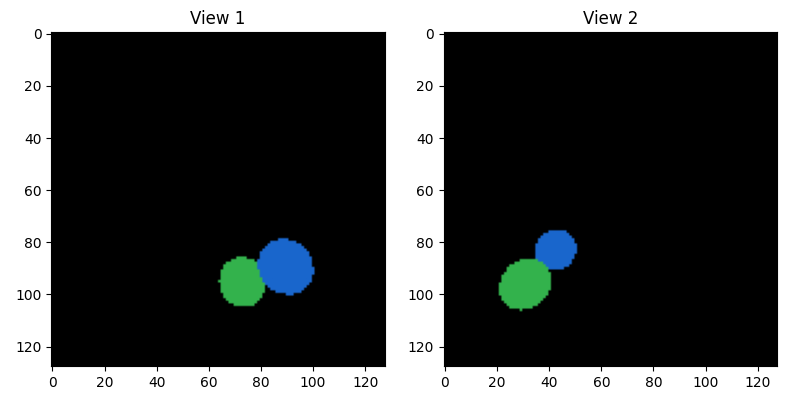
\includegraphics[width=0.5\textwidth]{sphere_tracing.png}
\caption{Rendered image from sphere tracing}
\end{figure}

\begin{figure}[H]
\centering
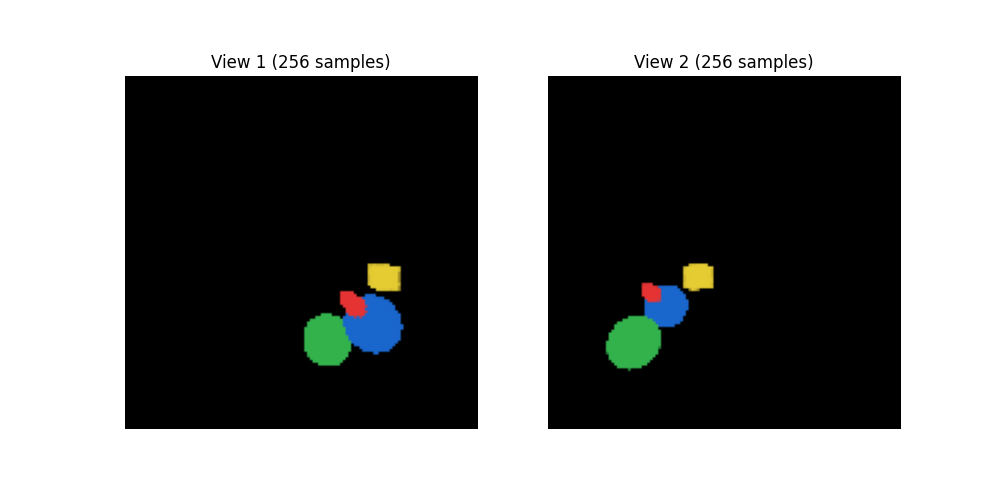
\includegraphics[width=0.5\textwidth]{volume_rendering.png}
\caption{Rendered image from volumetric rendering}
\end{figure}



\section{Answer to questions}
The reason why volumetric rendering is preferred to sphere tracing these days is mainly because volume-based methods are more robust. In volumetric rendering, the color is determined by summing over all the contributions along the marching ray, which is less prone to error if the geometry has very irregular shapes. In contrast, sphere tracing relies on finding the intersection point of the ray with the surface, which is more sensitive to the geometry of the scene. 




\end{document}

